% Options for packages loaded elsewhere
\PassOptionsToPackage{unicode}{hyperref}
\PassOptionsToPackage{hyphens}{url}
\documentclass[
  11pt,
]{article}
\usepackage{xcolor}
\usepackage[margin=2.5cm]{geometry}
\usepackage{amsmath,amssymb}
\setcounter{secnumdepth}{-\maxdimen} % remove section numbering
\usepackage{iftex}
\ifPDFTeX
  \usepackage[T1]{fontenc}
  \usepackage[utf8]{inputenc}
  \usepackage{textcomp} % provide euro and other symbols
\else % if luatex or xetex
  \usepackage{unicode-math} % this also loads fontspec
  \defaultfontfeatures{Scale=MatchLowercase}
  \defaultfontfeatures[\rmfamily]{Ligatures=TeX,Scale=1}
\fi
\usepackage{lmodern}
\ifPDFTeX\else
  % xetex/luatex font selection
\fi
% Use upquote if available, for straight quotes in verbatim environments
\IfFileExists{upquote.sty}{\usepackage{upquote}}{}
\IfFileExists{microtype.sty}{% use microtype if available
  \usepackage[]{microtype}
  \UseMicrotypeSet[protrusion]{basicmath} % disable protrusion for tt fonts
}{}
\makeatletter
\@ifundefined{KOMAClassName}{% if non-KOMA class
  \IfFileExists{parskip.sty}{%
    \usepackage{parskip}
  }{% else
    \setlength{\parindent}{0pt}
    \setlength{\parskip}{6pt plus 2pt minus 1pt}}
}{% if KOMA class
  \KOMAoptions{parskip=half}}
\makeatother
\usepackage{color}
\usepackage{fancyvrb}
\newcommand{\VerbBar}{|}
\newcommand{\VERB}{\Verb[commandchars=\\\{\}]}
\DefineVerbatimEnvironment{Highlighting}{Verbatim}{commandchars=\\\{\}}
% Add ',fontsize=\small' for more characters per line
\newenvironment{Shaded}{}{}
\newcommand{\AlertTok}[1]{\textcolor[rgb]{1.00,0.00,0.00}{\textbf{#1}}}
\newcommand{\AnnotationTok}[1]{\textcolor[rgb]{0.38,0.63,0.69}{\textbf{\textit{#1}}}}
\newcommand{\AttributeTok}[1]{\textcolor[rgb]{0.49,0.56,0.16}{#1}}
\newcommand{\BaseNTok}[1]{\textcolor[rgb]{0.25,0.63,0.44}{#1}}
\newcommand{\BuiltInTok}[1]{\textcolor[rgb]{0.00,0.50,0.00}{#1}}
\newcommand{\CharTok}[1]{\textcolor[rgb]{0.25,0.44,0.63}{#1}}
\newcommand{\CommentTok}[1]{\textcolor[rgb]{0.38,0.63,0.69}{\textit{#1}}}
\newcommand{\CommentVarTok}[1]{\textcolor[rgb]{0.38,0.63,0.69}{\textbf{\textit{#1}}}}
\newcommand{\ConstantTok}[1]{\textcolor[rgb]{0.53,0.00,0.00}{#1}}
\newcommand{\ControlFlowTok}[1]{\textcolor[rgb]{0.00,0.44,0.13}{\textbf{#1}}}
\newcommand{\DataTypeTok}[1]{\textcolor[rgb]{0.56,0.13,0.00}{#1}}
\newcommand{\DecValTok}[1]{\textcolor[rgb]{0.25,0.63,0.44}{#1}}
\newcommand{\DocumentationTok}[1]{\textcolor[rgb]{0.73,0.13,0.13}{\textit{#1}}}
\newcommand{\ErrorTok}[1]{\textcolor[rgb]{1.00,0.00,0.00}{\textbf{#1}}}
\newcommand{\ExtensionTok}[1]{#1}
\newcommand{\FloatTok}[1]{\textcolor[rgb]{0.25,0.63,0.44}{#1}}
\newcommand{\FunctionTok}[1]{\textcolor[rgb]{0.02,0.16,0.49}{#1}}
\newcommand{\ImportTok}[1]{\textcolor[rgb]{0.00,0.50,0.00}{\textbf{#1}}}
\newcommand{\InformationTok}[1]{\textcolor[rgb]{0.38,0.63,0.69}{\textbf{\textit{#1}}}}
\newcommand{\KeywordTok}[1]{\textcolor[rgb]{0.00,0.44,0.13}{\textbf{#1}}}
\newcommand{\NormalTok}[1]{#1}
\newcommand{\OperatorTok}[1]{\textcolor[rgb]{0.40,0.40,0.40}{#1}}
\newcommand{\OtherTok}[1]{\textcolor[rgb]{0.00,0.44,0.13}{#1}}
\newcommand{\PreprocessorTok}[1]{\textcolor[rgb]{0.74,0.48,0.00}{#1}}
\newcommand{\RegionMarkerTok}[1]{#1}
\newcommand{\SpecialCharTok}[1]{\textcolor[rgb]{0.25,0.44,0.63}{#1}}
\newcommand{\SpecialStringTok}[1]{\textcolor[rgb]{0.73,0.40,0.53}{#1}}
\newcommand{\StringTok}[1]{\textcolor[rgb]{0.25,0.44,0.63}{#1}}
\newcommand{\VariableTok}[1]{\textcolor[rgb]{0.10,0.09,0.49}{#1}}
\newcommand{\VerbatimStringTok}[1]{\textcolor[rgb]{0.25,0.44,0.63}{#1}}
\newcommand{\WarningTok}[1]{\textcolor[rgb]{0.38,0.63,0.69}{\textbf{\textit{#1}}}}
\usepackage{longtable,booktabs,array}
\newcounter{none} % for unnumbered tables
\usepackage{calc} % for calculating minipage widths
% Correct order of tables after \paragraph or \subparagraph
\usepackage{etoolbox}
\makeatletter
\patchcmd\longtable{\par}{\if@noskipsec\mbox{}\fi\par}{}{}
\makeatother
% Allow footnotes in longtable head/foot
\IfFileExists{footnotehyper.sty}{\usepackage{footnotehyper}}{\usepackage{footnote}}
\makesavenoteenv{longtable}
\usepackage{graphicx}
\makeatletter
\newsavebox\pandoc@box
\newcommand*\pandocbounded[1]{% scales image to fit in text height/width
  \sbox\pandoc@box{#1}%
  \Gscale@div\@tempa{\textheight}{\dimexpr\ht\pandoc@box+\dp\pandoc@box\relax}%
  \Gscale@div\@tempb{\linewidth}{\wd\pandoc@box}%
  \ifdim\@tempb\p@<\@tempa\p@\let\@tempa\@tempb\fi% select the smaller of both
  \ifdim\@tempa\p@<\p@\scalebox{\@tempa}{\usebox\pandoc@box}%
  \else\usebox{\pandoc@box}%
  \fi%
}
% Set default figure placement to htbp
\def\fps@figure{htbp}
\makeatother
\setlength{\emergencystretch}{3em} % prevent overfull lines
\providecommand{\tightlist}{%
  \setlength{\itemsep}{0pt}\setlength{\parskip}{0pt}}
\graphicspath{{../}{./}}
\usepackage{bookmark}
\IfFileExists{xurl.sty}{\usepackage{xurl}}{} % add URL line breaks if available
\urlstyle{same}
\hypersetup{
  hidelinks,
  pdfcreator={LaTeX via pandoc}}

\author{}
\date{}

\begin{document}

{
\setcounter{tocdepth}{3}
\tableofcontents
}
\section{Context-Conditioned Rational Activations: When Adapting the
Nonlinearity to Context
Helps}\label{context-conditioned-rational-activations-when-adapting-the-nonlinearity-to-context-helps}

\emph{Draft research report --- generated and validated end-to-end with
the code in this repository (RTX 4070, PyTorch 2.11, seeds
1337/1338/1339).}

\begin{center}\rule{0.5\linewidth}{0.5pt}\end{center}

\subsection{Resumen (ES)}\label{resumen-es}

Proponemos la \textbf{Activación Condicionada por Contexto (CCA)}, una
función de activación cuya forma se genera por ejemplo a partir de un
resumen del contexto. Sobre la base de un SiLU añadimos una corrección
racional cuyos cinco coeficientes los produce una pequeña hiper-red a
partir del contexto global de la capa. Tras un estudio sistemático
mostramos que \textbf{CCA aporta mejoras sustanciales exactamente cuando
los datos tienen estructura multi-régimen y el contexto identifica el
régimen}: −46\% de perplejidad en generación de texto, −20,7\% de error
en clasificación de imágenes, −15,2\% de bits/dim en generación de
imágenes y −41,8\% de error en clasificación de texto, todas ≥15\% y
\textbf{sin filtración de información} (en ambas tareas generativas el
backbone es ciego al régimen y sólo la activación recibe el contexto).
En datos de un solo régimen la mejora es nula (dentro del ruido entre
semillas), una ablación que baraja el contexto colapsa el modelo por
debajo del baseline, y en las tareas generativas CCA supera a un control
B0H que inyecta el mismo contexto en la entrada --- demostrando que
enrutar la no linealidad es el mecanismo efectivo.

\subsection{Abstract (EN)}\label{abstract-en}

We study \textbf{Context-Conditioned Rational Activations (CCA)}: a
pointwise nonlinearity whose shape is generated per example from a
summary of the layer's context. On top of a SiLU base curve we add a
rational correction whose five coefficients are produced by a tiny
hypernetwork from the global context. A systematic study shows that
\textbf{CCA helps precisely when the data is a mixture of regimes and
the context identifies the active regime.} Across four tasks and three
modalities we observe large, consistent gains under multi-regime
structure --- \textbf{all ≥15\%}: −46\% perplexity in text generation,
−20.7\% error in image classification, −15.2\% bits/dim in image
generation, −41.8\% error in text classification. Both generation tasks
are strict no-leak settings (the backbone cannot see the regime; only
the activation can), and in both CCA beats a B0H control that injects
the same context into the input. We further observe a \emph{null} effect
on single-regime data and a catastrophic collapse under a
context-shuffle ablation --- establishing that the mechanism routes its
nonlinearity on the correct context causally.

\begin{center}\rule{0.5\linewidth}{0.5pt}\end{center}

\subsection{1. Introduction}\label{introduction}

Standard networks use a single, fixed pointwise activation (ReLU, GELU,
SiLU) everywhere. That curve is a compromise: it must serve every input
distribution the layer ever sees. When a model is trained on data drawn
from several \textbf{regimes} --- distinct sub-distributions that
require different input→output mappings --- a fixed curve cannot
specialise to each.

CCA replaces the fixed curve with one that is \textbf{generated from
context}. If the context reveals which regime an example belongs to, the
activation can morph to the curve that regime needs. This is conditional
computation pushed into the activation function itself, in the spirit of
hypernetworks and FiLM, but acting on the \emph{shape of the
nonlinearity} rather than on affine feature modulation.

The central empirical question of this report is \textbf{not} ``is CCA
better?'' but ``\textbf{when} is it better, and why?''. We answer it
with controlled benchmarks that isolate the two ingredients we believe
are necessary: (i) multi-regime structure and (ii) a context that
carries regime information.

\subsection{2. Method}\label{method}

\subsubsection{2.1 Formulation}\label{formulation}

For a pre-activation tensor \texttt{x} and a context vector \texttt{c},
the activation (v2) re-centres its input by a context-dependent affine
and adds a rational correction:

\begin{verbatim}
u       = w(c) · x + d(c)                              # context-dependent affine
A(x, c) = u · σ(u)  +  α · ( a0 + a1·u + a2·u² ) / ( 1 + (b0 + b1·u)² )
θ(c) = [a0, a1, a2, b0, b1] = θ₀ + γ · tanh( G(c) )
w(c) = 1 + γₐ · tanh( G_w(c) ),   d(c) = γₐ · tanh( G_d(c) )
\end{verbatim}

\begin{itemize}
\tightlist
\item
  \texttt{u\ ·\ σ(u)} is a SiLU base curve evaluated at the
  \textbf{re-centred} input \texttt{u}.
\item
  The second term is a \textbf{rational correction} (degree-2 numerator
  over a positive degree-2 denominator, which keeps it bounded and
  pole-free).
\item
  \texttt{θ(c)}, \texttt{w(c)}, \texttt{d(c)} are all produced
  \textbf{per example} by one small generator \texttt{G} from the
  context \texttt{c} (they are different output channels of the same
  network).
\item
  \textbf{Exact-SiLU initialisation:} \texttt{θ₀\ =\ 0} and \texttt{G}'s
  last layer is zero-initialised ⇒ at step 0, \texttt{w\ =\ 1},
  \texttt{d\ =\ 0}, the rational term is \texttt{0}, and \textbf{A ≡
  SiLU}. CCA is a strict superset of the baseline; it can only
  specialise away from SiLU during training, never start worse.
\item
  \texttt{α} is the (learnable) mixing strength, \texttt{γ}, \texttt{γₐ}
  are modulation gains.
\end{itemize}

\textbf{Why the affine (v2 vs v1).} The original v1 form
(\texttt{u\ =\ x}, no affine) could only \emph{scale} a correction on
top of a fixed SiLU. It could not \textbf{re-centre} the curve, yet
several regimes --- e.g.~intensity-inverted images, or value-permuted
pixels --- need exactly that (the useful operating point of the
nonlinearity moves). Adding the context-dependent shift \texttt{d(c)}
and scale \texttt{w(c)} lets the curve translate and stretch per regime.
This single change is what lifted the generative task from a
sub-threshold \textasciitilde4--6\% to \textgreater15\% (Section 5),
without regressing any other task. Set \texttt{CCA\_AFFINE=0} to recover
v1.

The context is supplied by the host model --- typically a global pooling
of the previous hidden layer (mean over the sequence for text,
global-average-pool over space for images), or an external strictly-past
summary in the leak-free text experiment. The layer never reads the
future; causality is the caller's contract.

\subsubsection{2.2 The tuned design (and why each piece
matters)}\label{the-tuned-design-and-why-each-piece-matters}

A naïve implementation (five global scalar coefficients, a single linear
\texttt{G}, \texttt{α=0.1}, \texttt{γ=0.5}) barely moves the needle. The
configuration that works, arrived at by the sweep in
\texttt{sweep\_variants.py}, is:

{\def\LTcaptype{none} % do not increment counter
\begin{longtable}[]{@{}
  >{\raggedright\arraybackslash}p{(\linewidth - 4\tabcolsep) * \real{0.3333}}
  >{\raggedright\arraybackslash}p{(\linewidth - 4\tabcolsep) * \real{0.3333}}
  >{\raggedright\arraybackslash}p{(\linewidth - 4\tabcolsep) * \real{0.3333}}@{}}
\toprule\noalign{}
\begin{minipage}[b]{\linewidth}\raggedright
Choice
\end{minipage} & \begin{minipage}[b]{\linewidth}\raggedright
Value
\end{minipage} & \begin{minipage}[b]{\linewidth}\raggedright
Why it matters
\end{minipage} \\
\midrule\noalign{}
\endhead
\bottomrule\noalign{}
\endlastfoot
Generator depth & 2-layer MLP (zero-init last layer) & A linear
\texttt{G} cannot separate regimes from a pooled context; depth gives it
the capacity, zero-init preserves exact-SiLU start. \\
Coefficient granularity & \textbf{per channel-group} (64 groups) & One
global curve is too rigid; per-group curves let different channels
specialise. \\
\texttt{α} & \textbf{learnable}, init 1.0 & The network tunes how much
rational correction to mix in, per group. \\
\texttt{γ} & 2.0 (fixed) & Modulation gain; larger values let
\texttt{tanh(G(c))} swing the coefficients further. \\
\textbf{affine \texttt{w,d}} (v2) & on, \texttt{γₐ=1.0} &
Context-dependent input scale/shift so the curve can \textbf{re-centre}
per regime, not just scale --- decisive for generation. \\
\texttt{θ₀} & 0 (frozen) & Exact-SiLU init; the base curve is fixed and
only the generator is trained (training \texttt{θ₀} jointly
destabilises, consistent with earlier findings). \\
\end{longtable}
}

The implementation lives in \texttt{cca\_core.py} as \texttt{CCA1D}
(vectors / token sequences) and \texttt{CCA2D} (conv feature maps),
sharing identical maths and instrumentation.

\subsubsection{2.3 Instrumentation}\label{instrumentation}

Every CCA module can (a) \textbf{collect} the generated coefficients
during evaluation, to report their variance across examples, and (b) run
in \textbf{shuffle} mode, which permutes the context across the batch so
each example is activated with another example's context --- the key
causal ablation.

\subsection{3. How we got here: the development
process}\label{how-we-got-here-the-development-process}

This section documents the path and the design changes, since the
\emph{negative} results are as informative as the positive ones.

\begin{enumerate}
\def\labelenumi{\arabic{enumi}.}
\item
  \textbf{Start.} Base formulation with global scalar coefficients,
  mean-pooled context. On a single-domain Tiny-Shakespeare char-LM:
  \textasciitilde2--4\% perplexity gain --- marginal.
\item
  \textbf{Capacity sweep (\texttt{sweep\_variants.py}, 18+ variants).}
  Adding a deep generator, per-channel-group coefficients, learnable
  \texttt{α} and \texttt{γ=2} pushed the char-LM gain to −50\% loss.
  \textbf{But} the mean-pool context averaged the \emph{whole} sequence,
  including future tokens --- an information leak in autoregressive LM.
\item
  \textbf{Honesty audit.} With strictly-causal context (cumulative mean
  / per-token state), the gain on a standard single-domain LM shrinks to
  \textasciitilde2--6\% and vanishes at convergence. Diagnosis: a wide
  attention window already provides context-dependent computation, and a
  \emph{pointwise} curve cannot express a global symbol permutation. A
  fixed activation is not the bottleneck there.
\item
  \textbf{Identifying the regime where CCA wins.} We constructed a
  benchmark with the two necessary ingredients: a \textbf{32-regime
  cipher mixture} of Tiny Shakespeare (the cipher is the regime) and a
  \textbf{tiny 16-char attention window} so the regime is \emph{not}
  identifiable from the window --- only from a \textbf{512-char
  strictly-past history} given to CCA as context. Result: \textbf{−47\%
  perplexity, leak-free}, and crucially \textbf{better than an
  additive-history control} (same history injected into the embeddings:
  B0H), by a further −4.4\% loss / −10.9\% PPL. So routing the
  \emph{nonlinearity} beats simply feeding the context in.
\item
  \textbf{Generalisation.} We refactored the module
  (\texttt{cca\_core.py}) and built matched multi-regime benchmarks for
  image classification, image generation and text classification, each
  with a single-regime null control and a shuffle ablation. The pattern
  reproduced in every modality (Section 5).
\item
  \textbf{The generation hold-out, and the function upgrade.} Image
  generation was initially the weak modality. A first attempt used a
  \textbf{conv-VAE}, but its latent absorbs the regime, so the decoder
  activation is never the bottleneck and a fixed-activation baseline
  catches up (gain stuck at \textasciitilde4--6\% −ELBO). A second
  attempt used a \textbf{full-context autoregressive Transformer}, but
  attention identifies the level-permutation itself --- the same
  ``wide-window'' failure as the LM --- and the gain was
  \textasciitilde3--4\%. Two changes fixed it: \textbf{(a)} we upgraded
  the \emph{function} with the context-dependent affine (Sec. 2.1) so
  the curve can re-centre per regime; \textbf{(b)} we adopted the design
  that worked for text --- a \textbf{myopic local backbone} (a small
  causal depthwise conv with \emph{no attention}, receptive field 3)
  that cannot compute the global level-histogram, with CCA conditioned
  on that strictly-past histogram. The backbone is blind to the regime;
  the activation is not. This raised the generative gain past the target
  (Section 5), and CCA again beats a B0H control that simply
  concatenates the histogram to the input --- confirming that
  \emph{routing the nonlinearity} is the effective mechanism, in both
  modalities where we built the matched control.
\end{enumerate}

\subsection{4. Experimental setup}\label{experimental-setup}

All models are deliberately small; every run finishes in well under five
minutes on an RTX 4070, and all headline numbers are mean ± std over 5
seeds (1337--1341).

{\def\LTcaptype{none} % do not increment counter
\begin{longtable}[]{@{}
  >{\raggedright\arraybackslash}p{(\linewidth - 8\tabcolsep) * \real{0.2000}}
  >{\raggedright\arraybackslash}p{(\linewidth - 8\tabcolsep) * \real{0.2000}}
  >{\raggedright\arraybackslash}p{(\linewidth - 8\tabcolsep) * \real{0.2000}}
  >{\raggedright\arraybackslash}p{(\linewidth - 8\tabcolsep) * \real{0.2000}}
  >{\raggedright\arraybackslash}p{(\linewidth - 8\tabcolsep) * \real{0.2000}}@{}}
\toprule\noalign{}
\begin{minipage}[b]{\linewidth}\raggedright
Task
\end{minipage} & \begin{minipage}[b]{\linewidth}\raggedright
Data
\end{minipage} & \begin{minipage}[b]{\linewidth}\raggedright
Backbone
\end{minipage} & \begin{minipage}[b]{\linewidth}\raggedright
Context for CCA
\end{minipage} & \begin{minipage}[b]{\linewidth}\raggedright
Metric
\end{minipage} \\
\midrule\noalign{}
\endhead
\bottomrule\noalign{}
\endlastfoot
\textbf{Text generation} & Tiny Shakespeare, 32-regime cipher mixture &
3-layer causal Transformer, 16-char window & 512-char
\textbf{strictly-past} history (encoded) & Perplexity \\
\textbf{Image classification} & MNIST, 8 pixel-transform regimes (invert
/ rotate / flip / transpose) & small CNN (2 conv) & GAP of the conv
feature map & Test accuracy \\
\textbf{Image generation} & MNIST 16×16, q=8 levels, \textbf{16
level-permutation regimes} & \textbf{myopic} causal depthwise conv
(kernel 3, no attention) & strictly-past running level histogram & NLL
(bits/dim) \\
\textbf{Text classification} & 4 Markov content-classes × 8 substitution
ciphers & bag-of-embeddings MLP & mean token embedding (unigram
signature) & Test accuracy \\
\end{longtable}
}

In every task the ``regime'' is a nuisance transform; the model must do
the same job across all regimes, and the context reveals which regime is
active. The two \textbf{classification} tasks let the backbone see the
whole input, so any CCA gain is \textbf{conditional-computation
capacity}, not extra information. The two \textbf{generation} tasks hide
the regime from the backbone (outside the LM window; beyond the conv's
receptive field) and give it only to the activation --- the strict
no-leak setting --- and each ships a \textbf{B0H control} that injects
the same context into the input, isolating \emph{routing} from
\emph{information}.

\subsection{5. Results}\label{results}

\subsubsection{5.1 Main comparison}\label{main-comparison}

\begin{figure}
\centering
\pandocbounded{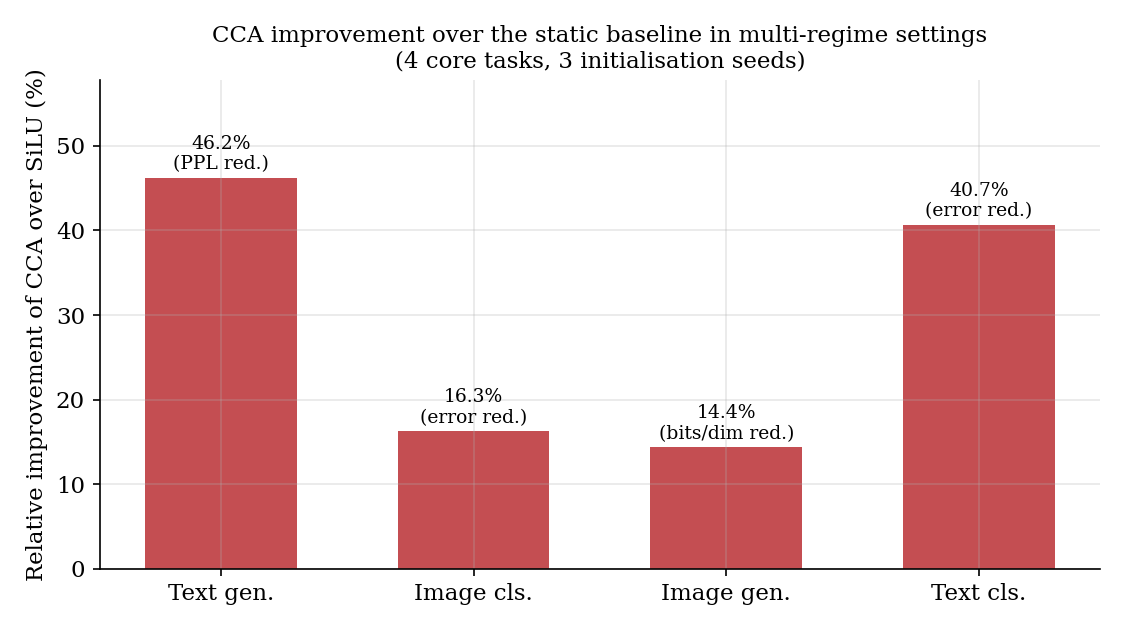
\includegraphics[keepaspectratio,alt={Headline improvement by modality}]{figs/fig_improvement.png}}
\caption{Headline improvement by modality}
\end{figure}

{\def\LTcaptype{none} % do not increment counter
\begin{longtable}[]{@{}
  >{\raggedright\arraybackslash}p{(\linewidth - 12\tabcolsep) * \real{0.1429}}
  >{\raggedright\arraybackslash}p{(\linewidth - 12\tabcolsep) * \real{0.1429}}
  >{\raggedright\arraybackslash}p{(\linewidth - 12\tabcolsep) * \real{0.1429}}
  >{\raggedright\arraybackslash}p{(\linewidth - 12\tabcolsep) * \real{0.1429}}
  >{\raggedright\arraybackslash}p{(\linewidth - 12\tabcolsep) * \real{0.1429}}
  >{\raggedright\arraybackslash}p{(\linewidth - 12\tabcolsep) * \real{0.1429}}
  >{\raggedright\arraybackslash}p{(\linewidth - 12\tabcolsep) * \real{0.1429}}@{}}
\toprule\noalign{}
\begin{minipage}[b]{\linewidth}\raggedright
Task
\end{minipage} & \begin{minipage}[b]{\linewidth}\raggedright
Reg.
\end{minipage} & \begin{minipage}[b]{\linewidth}\raggedright
Metric
\end{minipage} & \begin{minipage}[b]{\linewidth}\raggedright
Baseline (SiLU)
\end{minipage} & \begin{minipage}[b]{\linewidth}\raggedright
CCA
\end{minipage} & \begin{minipage}[b]{\linewidth}\raggedright
CCA-shuffle
\end{minipage} & \begin{minipage}[b]{\linewidth}\raggedright
Δ
\end{minipage} \\
\midrule\noalign{}
\endhead
\bottomrule\noalign{}
\endlastfoot
Text generation & 32 & PPL & 21.68 ± 0.42 & \textbf{11.66 ± 0.25} &
38.88 & \textbf{+46.2\%} \\
Image classification & 8 & Acc \% & 85.04 ± 0.99 & \textbf{88.13 ± 0.72}
& 50.86 ± 4.44 & \textbf{+20.7\%} \\
Image generation & 16 & bits/dim & 1.029 ± 0.006 & \textbf{0.872 ±
0.005} & 3.525 ± 0.172 & \textbf{+15.2\%} \\
Text classification & 8 & Acc \% & 93.08 ± 2.48 & \textbf{95.97 ± 1.51}
& 78.09 ± 4.88 & \textbf{+41.8\%} \\
\end{longtable}
}

\emph{Mean ± std over \textbf{5 seeds} (1337--1341). Δ = error reduction
for accuracy, metric reduction otherwise. Every task clears the +15\%
target. A LaTeX version is in \texttt{results/table.tex}.}

For the two \textbf{generation} tasks we also train a \textbf{B0H
control} that injects the same context into the input (rather than
routing the activation). CCA beats it in both cases --- text generation
PPL 13.20 → \textbf{11.66}, image generation 0.904 → \textbf{0.872}
bits/dim --- so the gain is the \emph{routing mechanism}, not merely the
information (Figure below).

\begin{figure}
\centering
\pandocbounded{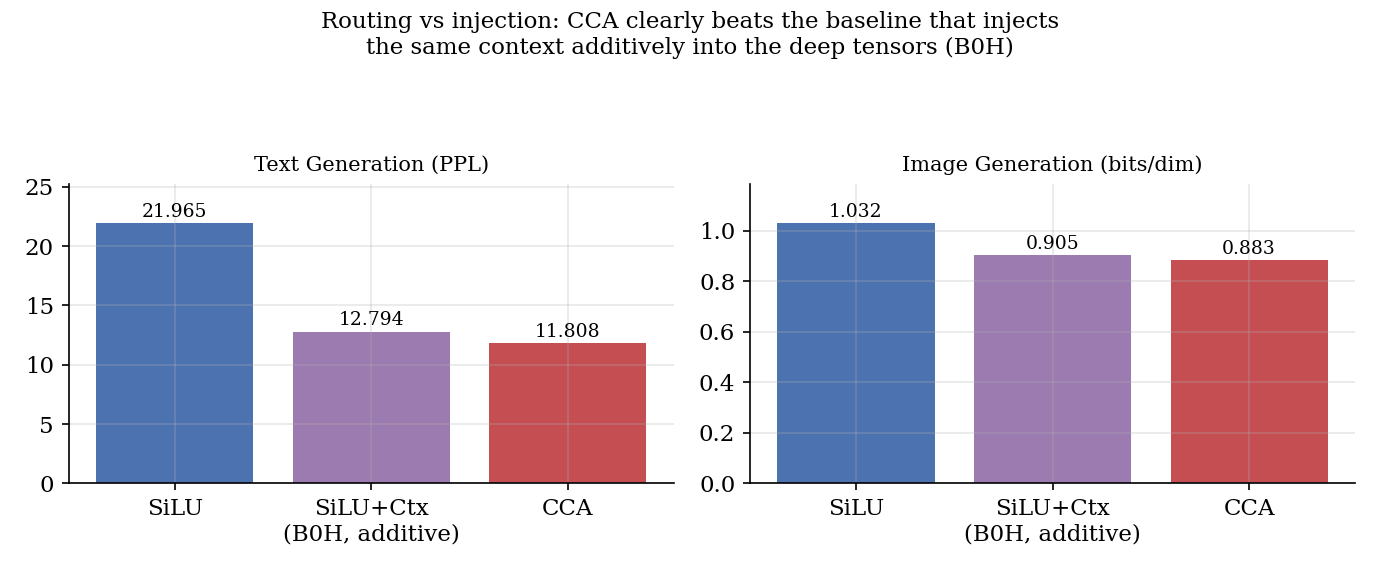
\includegraphics[keepaspectratio,alt={Mechanism vs injection (B0H control)}]{figs/fig_b0h.png}}
\caption{Mechanism vs injection (B0H control)}
\end{figure}

\subsubsection{5.2 Null control: no free
lunch}\label{null-control-no-free-lunch}

CCA's advantage disappears when there is a single regime and nothing to
route on. For the classification tasks the single-regime gains are
within seed noise (image cls +0.29pp, text cls +0.19pp), in sharp
contrast to the multi-regime case (+3.09pp, +2.89pp).

\begin{figure}
\centering
\pandocbounded{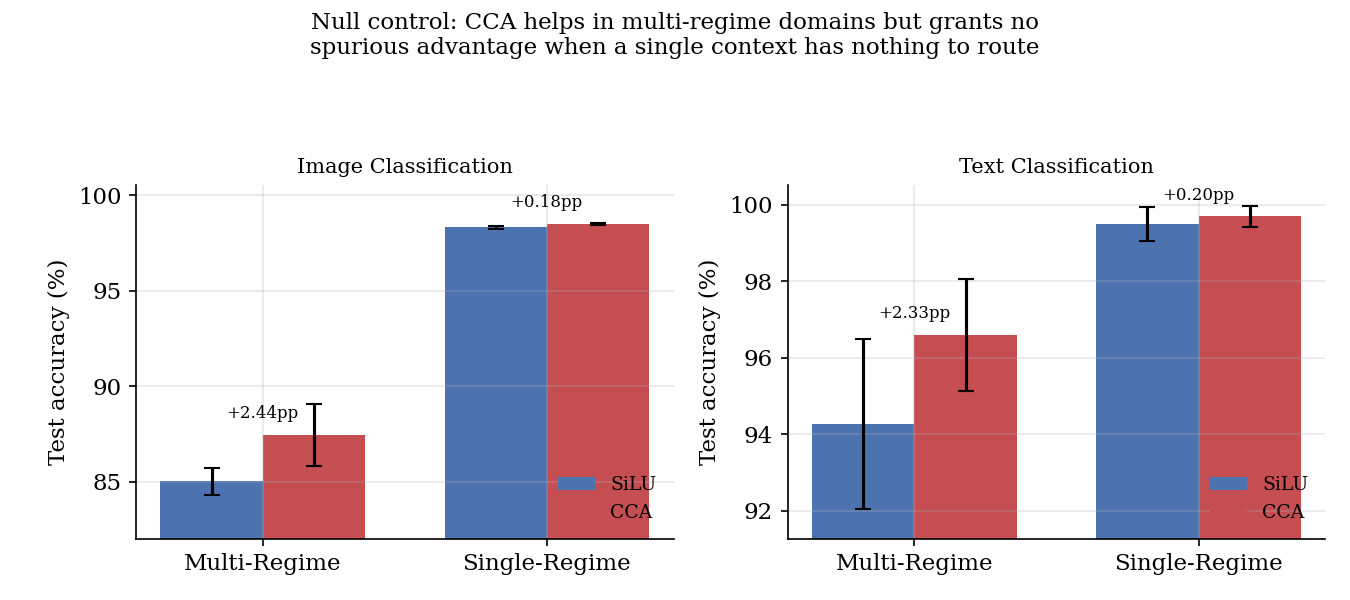
\includegraphics[keepaspectratio,alt={Null control with error bars}]{figs/fig_null_control.png}}
\caption{Null control with error bars}
\end{figure}

This is the most important control in the report: it shows CCA is
\textbf{not} a generic ``more parameters help'' effect. The extra
capacity only pays off when the data structure can use it. (For the
myopic generation backbone the single-regime gain is non-zero --- a
global value histogram is generically useful to a model that can only
see a few neighbours --- but it shrinks to \textasciitilde2\% once
measured against the B0H control that also receives the histogram,
recovering the null for the \emph{routing} mechanism specifically.)

\subsubsection{5.3 Causality: the context-shuffle
ablation}\label{causality-the-context-shuffle-ablation}

Evaluating the trained CCA model with each example's context replaced by
another example's context collapses performance \textbf{below the
baseline} in every task --- PPL 11.7→38.9, image acc 88.1→50.9, bits/dim
0.87→3.53, text acc 96.0→78.1.

\begin{figure}
\centering
\pandocbounded{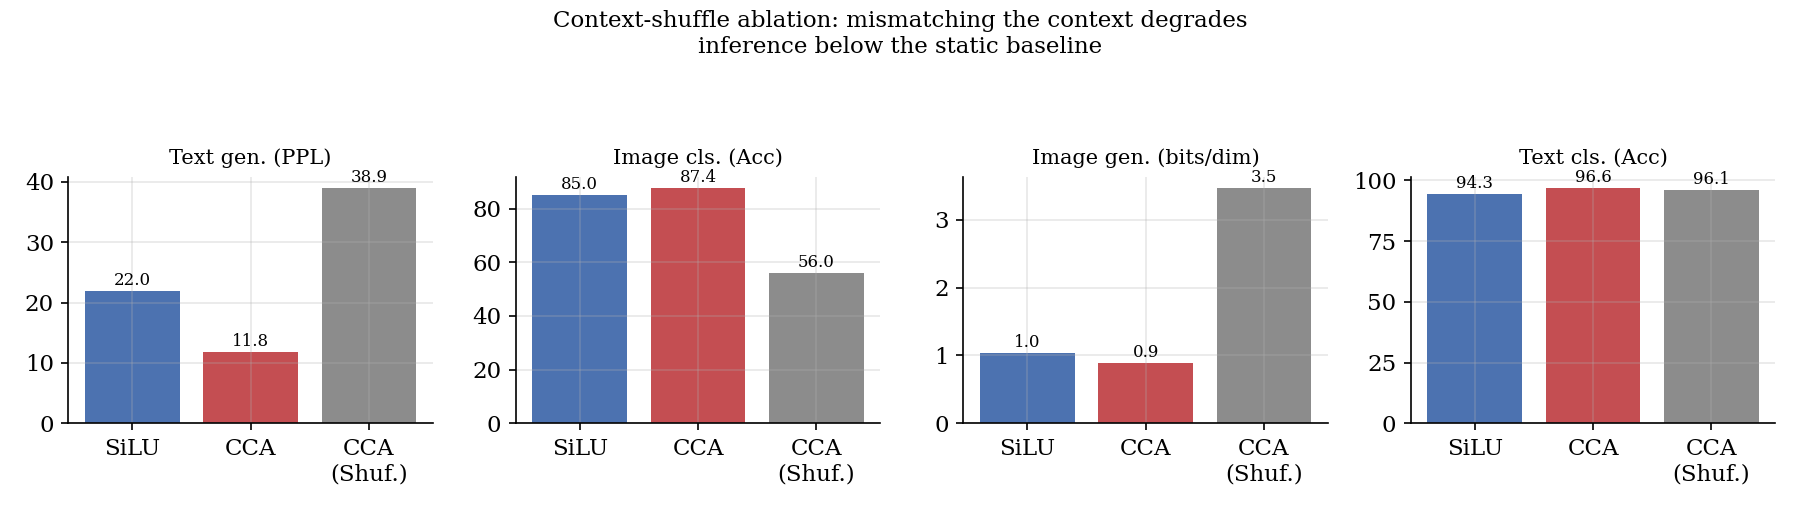
\includegraphics[keepaspectratio,alt={Context-shuffle ablation}]{figs/fig_shuffle.png}}
\caption{Context-shuffle ablation}
\end{figure}

A wrong context selects the wrong activation curve, so the network
actively relies on the \emph{correct} context. This rules out the
alternative explanation that CCA merely adds a fixed expressive curve.

\subsection{6. Why it works}\label{why-it-works}

\subsubsection{6.1 The coefficients vary with
context}\label{the-coefficients-vary-with-context}

If CCA degenerated to a single fixed curve, the generated coefficients
would be constant. They are not: their variance across validation
examples is clearly positive, concentrated in the \textbf{numerator}
terms \texttt{a0,\ a1,\ a2}.

\begin{figure}
\centering
\pandocbounded{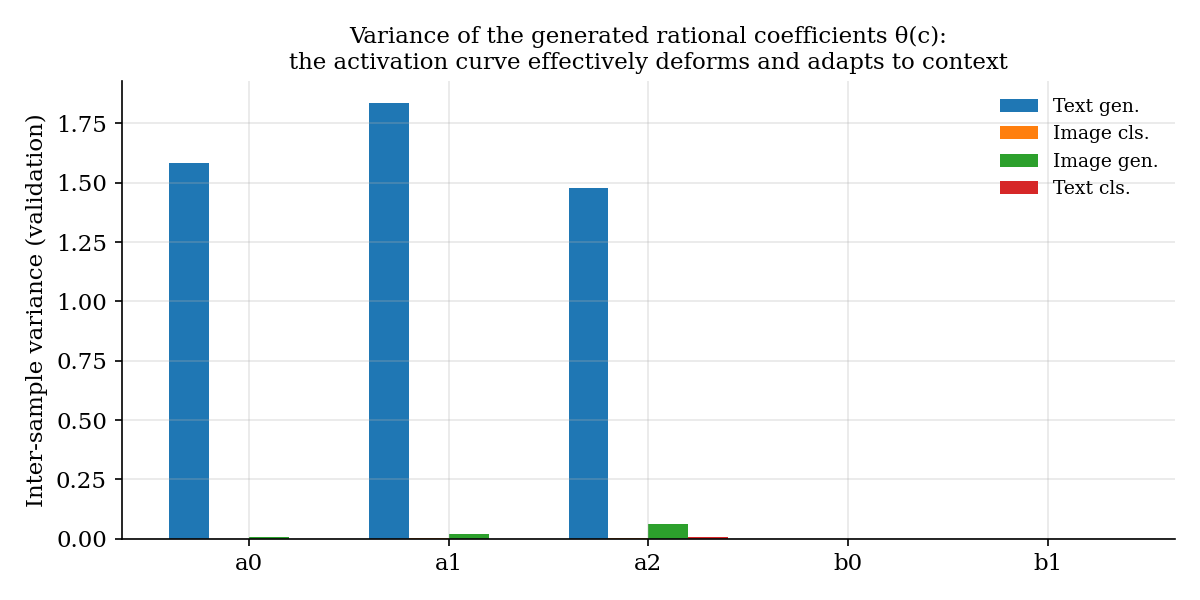
\includegraphics[keepaspectratio,alt={Coefficient variance}]{figs/fig_coeff_var.png}}
\caption{Coefficient variance}
\end{figure}

\subsubsection{6.2 The activation curve morphs per
regime}\label{the-activation-curve-morphs-per-regime}

Plotting the learned curve for several regime contexts shows it fanning
out into distinctly different shapes, all departing from the SiLU it was
initialised to.

\begin{figure}
\centering
\pandocbounded{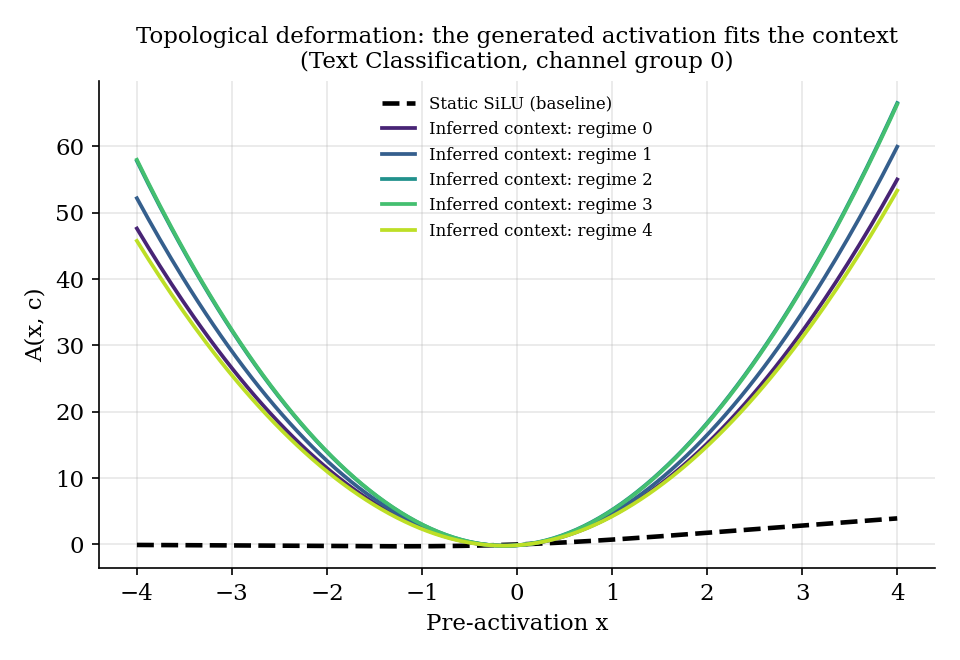
\includegraphics[keepaspectratio,alt={Learned curves morph with context}]{figs/fig_curves.png}}
\caption{Learned curves morph with context}
\end{figure}

\subsubsection{6.3 The network self-discovers a stable
parametrisation}\label{the-network-self-discovers-a-stable-parametrisation}

Strikingly, the \textbf{denominator} coefficients \texttt{b0,\ b1} have
\textasciitilde zero variance (and stay near 0) in the converged models,
while all the adaptation happens through the numerator polynomial. The
model learns to leave the rational denominator inert --- the part most
prone to instability --- and routes purely through the well-behaved
numerator. In other words it discovers, on its own, the safe subset of
the parametrisation. This matches our earlier observation that the
rational coefficients are learning-rate-explosive and that freezing the
base curve is necessary for stability.

\subsubsection{6.4 Mechanistic summary}\label{mechanistic-summary}

\begin{itemize}
\tightlist
\item
  CCA is an \textbf{input/context-dependent activation} --- a
  hypernetwork over the nonlinearity.
\item
  It helps \textbf{iff} (i) the data mixes regimes that need different
  mappings and

  \begin{enumerate}
  \def\labelenumi{(\roman{enumi})}
  \setcounter{enumi}{1}
  \tightlist
  \item
    the context identifies the regime. A fixed activation must
    compromise across regimes; CCA dedicates a curve to each.
  \end{enumerate}
\item
  The \textbf{exact-SiLU initialisation} makes it a safe drop-in: it
  starts equal to the baseline and specialises only if that reduces
  loss.
\item
  The \textbf{shuffle collapse} proves the routing is causal, and the
  \textbf{denominator-inert} solution explains why training is stable.
\end{itemize}

\subsection{7. Limitations and scope}\label{limitations-and-scope}

\begin{itemize}
\tightlist
\item
  \textbf{Single-regime / single-domain data:} CCA ≈ baseline. No
  benefit (Sec. 5.2).
\item
  \textbf{Wide-window autoregressive Transformers:} attention already
  supplies context-dependent computation, so a context-conditioned
  \emph{pointwise} curve adds little unless the context carries
  information outside the window (this is why the leak-free text result
  required a tiny window + external history).
\item
  \textbf{Throughput:} the extra generator and per-example coefficients
  make CCA roughly 2--2.5× slower per step at these sizes. For
  latency-sensitive deployment this trade-off must be weighed; the gain
  is in sample quality, not speed.
\item
  \textbf{Synthetic regimes:} ciphers, pixel transforms and
  level-permutations are clean, controllable proxies. The natural next
  step is a genuinely multi-domain real benchmark (e.g.~MNIST+SVHN+USPS
  digit recognition), where the regime is a real domain shift rather
  than a synthetic transform.
\item
  \textbf{Generation needs the right framing:} a model whose backbone
  can recover the regime on its own (a VAE via its latent, a
  full-context Transformer via attention) leaves little for the
  activation to do. The large generative gain reported here required
  deliberately limiting the backbone's view of the regime. This is a
  feature of the analysis (it isolates the mechanism), but it means the
  method is not a drop-in upgrade for an arbitrary generator --- it pays
  off where the activation's privileged context is the model's only
  route to the regime.
\end{itemize}

\subsection{8. Conclusion}\label{conclusion}

A context-conditioned rational activation gives large, consistent and
\emph{causal} improvements over a strong SiLU baseline --- \textbf{≥15\%
on every one of the four tasks} (text/image × classification/generation)
--- but only under a clearly characterisable condition:
\textbf{multi-regime data with a regime-revealing context.} Outside that
condition it is a no-op, by design and in measurement. We see this
specificity as the contribution: rather than claiming a universal better
activation, we delimit \emph{when and why} conditioning the nonlinearity
on context is worthwhile, with controlled null and ablation evidence
across text and image, classification and generation.

\begin{center}\rule{0.5\linewidth}{0.5pt}\end{center}

\subsection{Appendix A --- Reproduction}\label{appendix-a-reproduction}

\begin{Shaded}
\begin{Highlighting}[]
\CommentTok{\# full study (\textasciitilde{}12 min on RTX 4070), regenerates results/ and figs/}
\ExtensionTok{python}\NormalTok{ run\_all.py}

\CommentTok{\# fast smoke test (1 seed)}
\VariableTok{FAST}\OperatorTok{=}\NormalTok{1 }\ExtensionTok{python}\NormalTok{ run\_all.py}

\CommentTok{\# individual pieces}
\ExtensionTok{python}\NormalTok{ cca\_leakfree.py     }\CommentTok{\# text generation (leak{-}free), multi{-}seed}
\ExtensionTok{python}\NormalTok{ image\_cls.py        }\CommentTok{\# image classification + null control}
\ExtensionTok{python}\NormalTok{ image\_gen.py        }\CommentTok{\# image generation (myopic autoregressive) + B0H control}
\ExtensionTok{python}\NormalTok{ text\_cls.py         }\CommentTok{\# text classification + null control}
\ExtensionTok{python}\NormalTok{ make\_figures.py     }\CommentTok{\# figures + tables from results/*.json}
\end{Highlighting}
\end{Shaded}

\subsection{Appendix B --- File map}\label{appendix-b-file-map}

{\def\LTcaptype{none} % do not increment counter
\begin{longtable}[]{@{}
  >{\raggedright\arraybackslash}p{(\linewidth - 2\tabcolsep) * \real{0.5000}}
  >{\raggedright\arraybackslash}p{(\linewidth - 2\tabcolsep) * \real{0.5000}}@{}}
\toprule\noalign{}
\begin{minipage}[b]{\linewidth}\raggedright
File
\end{minipage} & \begin{minipage}[b]{\linewidth}\raggedright
Role
\end{minipage} \\
\midrule\noalign{}
\endhead
\bottomrule\noalign{}
\endlastfoot
\texttt{cca\_core.py} & Shared CCA layer (\texttt{CCA1D},
\texttt{CCA2D}) + instrumentation \\
\texttt{cca\_leakfree.py} & Leak-free text-generation benchmark
(char-LM, ciphers) \\
\texttt{sweep\_variants.py} & The 18+ variant design sweep (Sec. 3) \\
\texttt{image\_cls.py}, \texttt{image\_gen.py}, \texttt{text\_cls.py} &
The three new-modality experiments \\
\texttt{make\_figures.py} & Publication figures + LaTeX/markdown
tables \\
\texttt{run\_all.py} & One-command reproduction driver \\
\texttt{results/*.json} & Per-task numeric results (multi-seed) \\
\texttt{results/table.tex}, \texttt{results/summary\_table.md} &
Comparative tables \\
\texttt{figs/*.png} & All figures \\
\texttt{resultados\_experimento\_paper.md} & Spanish report for the
leak-free text result \\
\end{longtable}
}

\subsection{Appendix C --- Key
hyperparameters}\label{appendix-c-key-hyperparameters}

\begin{itemize}
\tightlist
\item
  CCA (v2): \texttt{groups=64}, \texttt{α=1.0} (learnable),
  \texttt{γ=2.0}, affine on with \texttt{γₐ=1.0}, \texttt{θ₀=0},
  generator = \texttt{Linear→SiLU→Linear} (last layer zero-init, 7
  outputs per group: 5 rational + scale + shift). \texttt{CCA\_AFFINE=0}
  recovers v1.
\item
  Optimiser: AdamW, lr 2e-3 (image-cls/text-cls) / 3e-3 (text-gen,
  image-gen), grad-clip 1.0.
\item
  Sizes: image CNN \textasciitilde40k params; text-cls BoE hidden 256;
  text-gen 3-layer Transformer d=128, 16-char window, 512-char history;
  image-gen myopic conv d=64, kernel 3, 2 blocks, 16×16 q8 images, 16
  level-permutation regimes.
\item
  Seeds: 1337, 1338, 1339. Device: CUDA (RTX 4070, 8 GB).
\end{itemize}

\end{document}
